\documentclass[a4paper, twoside]{report}

%% Language and font encodings
\usepackage[english]{babel}
\usepackage[utf8x]{inputenc}
\usepackage[T1]{fontenc}

%% Sets page size and margins
\usepackage[a4paper,top=2cm,bottom=2.5cm,left=2cm,right=2cm,marginparwidth=1cm]{geometry}

%% Useful packages
\usepackage{amsmath}
\usepackage{graphicx}
\usepackage{subcaption}
\usepackage{listings}
\usepackage{color}
\usepackage{float}
\usepackage{caption}
\lstset{basicstyle=\small\ttfamily,
    keywordstyle=\color{purple}}
\usepackage{tikz}
\usetikzlibrary{calc,positioning,shapes,arrows}
\usepackage{tabularx}
\newcolumntype{L}{>{\hsize=0.7\hsize\raggedright\arraybackslash}X}
\newcolumntype{H}{>{\raggedright\arraybackslash}X}
\def\arraystretch{1.2}
\usepackage{booktabs}
\usepackage[colorinlistoftodos]{todonotes}
\usepackage[colorlinks=true, allcolors=blue]{hyperref}
\usepackage{enumitem}
\setlist[enumerate]{leftmargin=*}



\title{Building an Efficient Query Processor \\ by Generating OpenCL Code \\ from Voodoo Vector Algebra}
\author{Alexander Clarke \\ Qiang Feng \\ Mayeul Fournial \\ Pranav Kalidindi \\ Jordan Spooner \\ Laurence Squires}
% Update supervisor and other title stuff in title/title.tex

%% Our own style changes
\setlength{\parindent}{0pt}
\setlength{\parskip}{\medskipamount}
\usepackage{tgpagella}

\begin{document}
\input{title/title.tex}

\renewcommand{\abstractname}{Acknowledgements}
\begin{abstract}
We would like to thank Holger Pirk for his continuous guidance and support. We would also like to thank Robert Chatley for the invaluable advice from each of our software engineering consultations.
\end{abstract}

\tableofcontents

\chapter{Executive Summary}

\paragraph{Background}

Query performance in most popular relational databases is largely determined by CPU costs, and performance tends to be poor on modern CPUs as a result of poor locality and branch predictability.

\emph{Voodoo} \cite{Pirk:2016:VVA:3007328.3007336} is a vector algebra which can be used as a easily optimisable intermediate representation for database queries. An existing database back-end using a Voodoo IR has been shown to generate highly efficient OpenCL code for queries, often outperforming existing state-of-the-art in-memory query processors.

\paragraph{Problems}

However, the existing implementation consisted of several disjoint components, and only supported queries in the TPC-H benchmark, whose plans were hardcoded into the driver program - i.e. it was not possible to run arbitrary queries. As such, it would be difficult for researchers to explore and use Voodoo.

Furthermore, the code generation itself was complex and fragile, making it difficult for researchers to ensure its correctness, or extend the Voodoo kernel in any useful way.

\paragraph{Achievements}

We have made Voodoo more accessible to researchers, who will be able to set up and begin using Voodoo more easily. They can view the logical plan, Voodoo algebra and OpenCL code for an SQL query, as well as the results of its execution, using just a simple JDBC client.

Additionally, researchers will find it easier to to maintain and extend Voodoo, as a result of the almost entirely new implementation of the Voodoo kernel we have written, which uses an AST to generate simpler, but in most cases, similarly efficient code.

\paragraph{Applications}

We expect the main users of our work to be researchers, who might want to use Voodoo to express optimisations for main-memory query processors. We believe we have made it easier for them to use and extend Voodoo.

Of course, high-performance in-memory databases also have many applications in industry, and a database using a Voodoo IR could be particularly useful when query processing time is a major concern, such as in real-time or scientific applications. We have developed what is effectively a simple DBMS based on Voodoo algebra, which could form a strong starting-point for such a system.

\chapter{Introduction}

\section{Motivation}

Most of today's popular relational databases use a \emph{Volcano}-style iterator model \cite{Graefe:1994:VEP:627290.627558} for query processing. In this processing model, each operator (say, a projection, selection, join, etc.) produces a stream of tuples. The output stream of another operator is consumed using a simple interface, consisting only of the functions \texttt{open()}, \texttt{next()} and \texttt{close()}.

\begin{figure}
\centering
\begin{subfigure}[b]{0.45\textwidth}
    \centering
    \begin{lstlisting}[language=SQL]
SELECT
  "c_nationkey",
  COUNT("c_custkey")
    AS "customers_in_debt"
FROM
  "customer"
  JOIN "nation"
    ON "c_nationkey" = "n_nationkey"
WHERE
  "c_acctbal" < 0 
GROUP BY
  "c_nationkey"
    \end{lstlisting}
    \caption{A simple SQL query}
    \label{fig:simple-query}
\end{subfigure}
\begin{subfigure}[b]{0.45\textwidth}
    \centering
    \begin{overpic}[scale=0.205]{introduction/volcano.pdf}
        \put(0, 0) {
            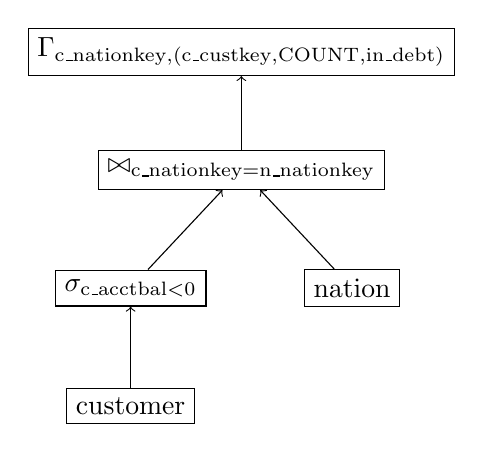
\begin{tikzpicture}[nodes={draw, rectangle}, sibling distance=80pt, <-]
                \node{$\Gamma_{\text{c\_nationkey}, (\text{c\_custkey}, \text{COUNT}, \text{in\_debt})}$}
                    child{node{$\bowtie_{\text{c\_nationkey} = \text{n\_nationkey}}$}
                        child{node{$\sigma_{\text{c\_acctbal} < 0}$}
                            child{node{customer}}}
                        child{node{nation}}};
            \end{tikzpicture}
        }
    \end{overpic}
    \caption{Evaluating \ref{fig:simple-query} using Volcano processing}
    \label{fig:volcano-processing}
\end{subfigure}
\\[5ex]
\begin{subfigure}[b]{0.45\textwidth}
    \centering
    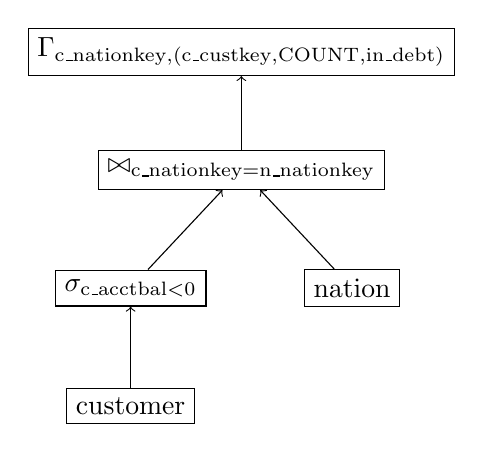
\begin{tikzpicture}[nodes={draw, rectangle}, sibling distance=80pt, <-]
        \node{$\Gamma_{\text{c\_nationkey}, (\text{c\_custkey}, \text{COUNT}, \text{in\_debt})}$}
            child{node{$\bowtie_{\text{c\_nationkey} = \text{n\_nationkey}}$}
                child{node{$\sigma_{\text{c\_acctbal} < 0}$}
                    child{node{customer}}}
                child{node{nation}}};
    \end{tikzpicture}
    \caption{Evaluating \ref{fig:simple-query} using bulk processing}
    \label{fig:bulk-processing}
\end{subfigure}
\begin{subfigure}[b]{0.45\textwidth}
    \centering
    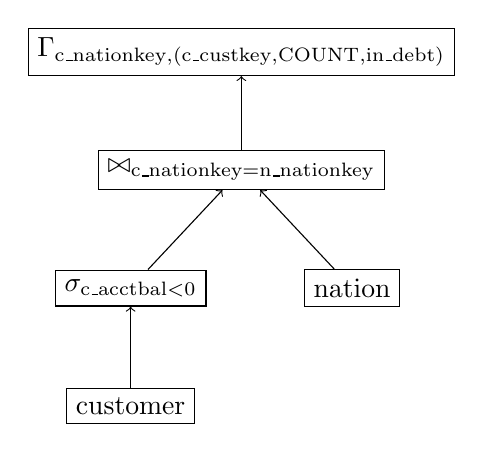
\begin{tikzpicture}[nodes={draw, rectangle}, sibling distance=80pt, <-]
        \node{$\Gamma_{\text{c\_nationkey}, (\text{c\_custkey}, \text{COUNT}, \text{in\_debt})}$}
            child{node{$\bowtie_{\text{c\_nationkey} = \text{n\_nationkey}}$}
                child{node{$\sigma_{\text{c\_acctbal} < 0}$}
                    child{node{customer}}}
                child{node{nation}}};
    \end{tikzpicture}
    \caption{Evaluating \ref{fig:simple-query} using code generation}
    \label{fig:code-generation}
\end{subfigure}
\caption{Approaches for improving query processing time}
\end{figure}

Whilst these databases benefit from a clean and flexible design which maximises maintainability and developer productivity, the Volcano-style processing model makes excessive use of function calls. For example, consider alone the \texttt{next()} call, which must be made for every tuple in the input, each intermediate result, and the final result. As main memory has grown, CPU costs now tend to be the query processing, and these function calls lead to frequent instruction mispredictions, and by extension control hazards, requiring CPU stalls which significantly degrade performance.

Database systems such as \emph{MonetDB} \cite{Boncz:2008:BMW:1409360.1409380} pioneered a bulk-processing approach, in which instead of considering one tuple at a time, entire columns are considered at a time. By doing so, the cost of calling the next operator is amortised over the number of tuples. However, this approach introduces a new cost: intermediate results must now be materialised. Whilst the iterator-model can pipeline most operators (that is, the output of one operator can be passed directly to the input of the next), this is no longer possible with the bulk-processing model, which must make all resulting tuples accessible to the next operator to process at once. This often results in memory bandwidth constraining performance.

In an attempt to solve this, a new query engine, \emph{X100} \cite{DBLP:conf/cidr/BonczZN05} (which later evolved into VectorWise), was built for MonetDB, which processes smaller (say 1000-value) vectors, which form chunks of columns. These vectors can fit in the CPU cache, and can be pipelined to avoid expensive materialisation.

More recently, the \emph{HyPer} in-memory database system \cite{Neumann:2011:ECE:2002938.2002940} was shown to significantly outperform MonetDB and VectorWise in most cases, by using LLVM to compile queries into machine code with better locality and a more predictable branch layout. In this approach, chains of operators which can be pipelined (i.e. chains that do not require materialisation) are identified, and each of these fragments is compiled separately into machine code. This reverses the direction of data-flow control: instead of each operator asking its input for tuples, each fragment of code processes the data and makes it available to the next fragment. Operators within each fragment leave tuples inside the CPU registers and so are extremely cheap, whilst pipeline-breaking operators (at the edge of fragments) would have required materialisation anyway, so there is no significant performance implication for them.

\emph{Voodoo} \cite{Pirk:2016:VVA:3007328.3007336} is a vector algebra which can be used as an intermediate representation between a database query and a code implementation, similar to what HyPer might produce. Voodoo allows the often data and hardware dependant kind of optimisations used in systems such as HyPer to be expressed in a portable way, and is designed to be \emph{tunable}, that is, it is able to express very simply most optimisations for in-memory query processing. It has been shown to generate highly-efficient OpenCL code to run on GPUs, outperforming existing state-of-the-art in-memory query processors for many queries.

Whilst benchmarks have shown that using Voodoo allows some of the fastest query processing times out of any modern approach, it was not really available in a form that made it easy to use:

\begin{enumerate}
    \item The existing Voodoo implementation was used as a replacement back-end for MonetDB. However the components to convert a query to a MonetDB plan and a MonetDB plan to Voodoo algebra remained mostly separate to the Voodoo kernel (code generator) itself, so there was no way to run queries, apart from TPC-H benchmarking queries whose plans were hard-coded into the driver program.
    \item The code generation itself was done by concatenating strings which formed the OpenCL program. This approach resulted in complex and fragile code, which was very difficult to extend. Importantly, once code had been written to the string, it became extremely difficult to change or move.
    \item Certain parts of the code also suffered from particularly sparse documentation, and several bugs which were identified during this project.
\end{enumerate}

\section{Objectives}

Main goal: make this usable for researchers: provide a front-end to what was just a benchmarking application, improve code generation...

1. Build a front-end to get SQL -> Logical plan -> Vooodoo for arbitrary schema, query.

2. Generate code using AST, to improve readability of generated code, and ease of implementation.

\section{Achievements}

Use \url{https://docs.google.com/document/d/1tCYCOFDeL8E3USIOunRNrqh6ekP_-kAQVHMrNJ4jk04} for achievments. Try to back everything up in a quantifiable way...

% We have developed a front-end for the Voodoo kernel, which allows for arbitrary queries to be run through a single program. In addition to this, we have provided a CI setup which demonstrates a provably correct setup for building the database system. We claim that this has made Voodoo much more accessible to researchers, who will be able to set up and begin to use Voodoo much more easily. They can connect to Voodoo using JDBC, and view the logical plan, Voodoo algebra and OpenCL code for a query, as well as the results of its execution.

% Furthermore, we have written a new implementation for the Voodoo kernel that uses an AST to generate OpenCL code. This implementation is less fragile and complex than the existing string-based implementation. We claim that it produces simpler code with performance roughly comparable to the existing implementation in most cases. We believe that it also significantly improves the extensibility of the Voodoo kernel.

1. Document and formalise installation...

1a. Contribute bugfixes required to get code to compile and run, update documentation

1b. Provide a dockerfile that prescribes the required setup

1c. Introduce CI that ensures the project can always build

2. Develop Calcite adapter that supports these SQL queries...

2a. Support arbitrary schemas with these types compared to before...

2b. Support arbitrary queries using these logical operators compared to before...

2c. Support rule-based logical optimisations using Calcite...

2d. Support enumerable operators using Calcite...

2e. Support integration with C++ printer implementation...

2f. Support integration with C++ AST implementation, by extending API...

2g. Provide a JDBC connection through Calcite

(2h. Provide a front-end that demonstrates the full process).

3. Develop a Clang-AST based implementation of Voodoo API.

3a. Support these Voodoo operators compared to before...

3b. Improve quality of implementation code as measured by this metric...

3c. Improve quality of generated code as measured by this metric...

3d. Improve ease-of-use as demonstrated by example (cross?), by providing AST components...

3e. Support future extension to C-like languages such as CUDA through generic processing class...

\chapter{Project Management}

Use \url{https://docs.google.com/document/d/1tCYCOFDeL8E3USIOunRNrqh6ekP_-kAQVHMrNJ4jk04} to complete. Add screenshots/photos wherever possible...

\section{Project planning}

We originally decided on these checkpoint goals...
But actually achieved...

We split our work using GitLab issues, assigned to any group member...

We had these GitLab tags to keep track of issues in different milestones...

We attempted to split work equally, these were each person's main contributions...

\section{Project organisation}

We used eXtreme programming which means...

Meetings with Holger treated as iteration meetings, work estimation and backlog grooming...

Standups for more frequent communication...

Slack for all other communication, we used these channels...

\section{Software engineering practices}

Pair programming...

Use of Git, branching...

Testing...

CI...

PRs, requiring approval for pushes to Voodoo and Calcite repos...

\chapter{Design and Implementation}

\section{Architectural overview}

\begin{figure}[H]
\includegraphics[width=\linewidth]{design-and-implementation/representations.pdf}
\centering
\caption{Translation process from an SQL query to OpenCL code}
\label{fig:translation-process}
\end{figure}

Figure \ref{fig:translation-process} shows our overall approach to processing a query. Starting with an SQL query, we first generate a logical plan, consisting of relational algebra expressions. These relational algebra expressions are then translated to Voodoo vector algebra. An abstract syntax tree is built up from the Voodoo vector algebra, and this AST is then used to generate OpenCL code, which we then run to produce a final result. Appendix \ref{appendix:full-query} shows an example of a query going through this full process.

The dashed lines in figure \ref{fig:translation-process} show the existing approach, preceding our work. This included a comprehensive plan compiler, able to process MonetDB plans, and an implementation of Voodoo, which translated Voodoo vector expressions directly to OpenCL code, using string streams. As shown, our approach represents an almost entirely new implementation. The benefit of this is that we are able to provide an interactive SQL front-end and a more versatile approach to code generation.

We use various frameworks and technologies to implement our approach, some of which are described in section \ref{section:tech}. Figure \ref{fig:voodoo-architecture} provides an overview of the full architecture. Elements in purple represent parts of the architecture which we have implemented, whilst blue elements represent components of the frameworks, libraries, or existing code which we heavily use.

In brief, translation from an SQL query to Voodoo API calls is done in Java, by building on top of the Apache Calcite framework. This involves implementing an adapter to handle data access and processing, which we describe in detail in section \ref{section:sql-to-voodoo}. Translation from Voodoo to OpenCL is done in C++, and makes use of Clang. Here, we have developed from scratch an implementation of the Voodoo API, which we discuss in section \ref{section:voodoo-to-opencl}.

\begin{figure}[p]
\vspace*{-1.4cm}
\makebox[\linewidth]{
    \includegraphics[width=1.1\linewidth]{design-and-implementation/project-architecture.pdf}
}
\centering
\vspace*{-0.7cm}
\caption{An architectural overview of our Voodoo-based query processor}
\label{fig:voodoo-architecture}
\end{figure}

\section{Technical background}
\label{section:tech}

\subsection{Voodoo}\label{original-voodoo-impl}

As we discussed in the introduction, \emph{Voodoo} \cite{Pirk:2016:VVA:3007328.3007336} is a vector algebra which can be used as an intermediate representation between a database query and generated code for that query. It consists of functions defining vector operations, such as the binary operations \texttt{Add} or \texttt{LogicalAnd}, and more complex or specific operations such as \texttt{Gather}, \texttt{Zip} and \texttt{FoldMin} (which are explained in detail in appendix \ref{appendix:api}). A sequential aggregation query is shown in figure \ref{fig:short-query}, which sums the balance of all the bank accounts with more than £10,000 on them. The corresponding (simplified) Voodoo program would load the column of the table in memory, filter the column according to the fixed predicate and then aggregate it.

\begin{figure}[h]
    \centering
\begin{subfigure}[h]{0.39\textwidth}
    \centering
\begin{lstlisting}[language=SQL]
SELECT SUM("account_balance")
FROM account
WHERE account_balance > 10000
\end{lstlisting}
    %\caption{Evaluating \ref{fig:simple-query} using bulk processing}
    \label{fig:short-query-sql}
\end{subfigure}
\begin{subfigure}[h]{0.59\textwidth}
    \centering
\begin{lstlisting}
balance = Load("account_balance")
big_balances = Greater(balance, 10000)
aggregated_balances = FoldSelect(big_balances)
result = FoldSum(aggregated_balances)
\end{lstlisting}
    \label{fig:short-query-vdl}
\end{subfigure}
    \caption{An intuition on Voodoo (ignoring keypaths, some vectors not shown)}
    \label{fig:short-query}
\end{figure}

The existing Voodoo implementation (which we will often refer to as the \emph{back-end}) included a high-performance database \emph{kernel}\footnote{We use kernel to refer to the query processing engine at the core of the database, here the part that evaluates Voodoo expressions.} written in C++ that implemented the \texttt{VoodooAPI} (an interface of the different vector functions in Voodoo). This implementation is called the original \texttt{OpenCL} back-end as opposed to the new \texttt{ClangAST} back-end (which also generates OpenCL). The former can generate and run the OpenCL code for the TPC-H queries\footnote{The TPC-H Benchmark is an industry-standard benchmark for comparing the OLAP performance of database systems. It consists of a set of complex queries that run on a specific single databases schema. The full specification is available at \url{http://www.tpc.org/TPC_Documents_Current_Versions/pdf/tpc-h_v2.17.3.pdf}.}, which Voodoo representation (the \texttt{VoodooAPI} calls) where being given to the \texttt{OpenCL} back-end or derived from a MonetDB plan (see Figure \ref{fig:translation-process}). The data was loaded from a MonetDB datafarm that was set up separately and loaded in memory before running the queries. There was notably another implementation of the \texttt{VoodooAPI}, called the \texttt{Printer}, that proved useful when debugging the front-end. This implementation prints the Voodoo programs as the Voodoo functions were called instead of actually evaluating anything. Figure \ref{fig:voodoo-architecture} shows how the \textt{VoodooAPI} and existing implementations fit into our overall architecture.

\subsection{Apache Calcite}

\emph{Apache Calcite} \cite{Begoli:2018:ACF:3183713.3190662} is a software framework that provides query language support, query optimisation and query processing, and is used by several popular data processing systems, particularly those in the Hadoop ecosystem. We use it mainly to translate SQL queries to a Voodoo implementation (described in section \ref{section:sql-to-voodoo}).

Whilst Calcite is written entirely in Java, which ocassionally makes interaction with the Voodoo kernel difficult, Calcite was chosen as the framework on which to develop our front-end, for the following reasons:

\begin{enumerate}
    \item Calcite is fairly widely adopted, and with this comes open-source friendliness and stability. In our use of Apache Calcite during this project, we have only encountered two critical unresolved bugs.
    \item By building on top of Calcite, we benefit from not having to entirely implement SQL parsing and validation, JDBC compliancy, and default operator implementations (which are useful when the Voodoo implementation of an operator would be beyond the scope of this project) ourselves.
\end{enumerate}
 
From this point, we assume a comprehensive understanding of the Apache Calcite framework, which is described in detail in appendix \ref{appendix:calcite}.

\subsection{SWIG\label{swig}}

The Simplified Wrapper and Interface Generator (\emph{SWIG}) \cite{Beazley:1996:SEU:1267498.1267513} allows the call to native C++ function in various languages and in particular Java. It requires to write an interface file containing the list of existing C++ classes, types, and methods we want to expose to Java that SWIG will then compile.

In our case, SWIG generates both a \emph{Java Native Interface} (JNI) shared library from compiling the exposed C++ code along with a corresponding JAR that contains the corresponding Java classes, types and methods that we can use as an external library in Calcite. SWIG handles most of the harmonisation between C++ and Java like respecting C++ virtual function calls, class inheritance, handling pointers, memory ownership (the most simple generated Java classes are in fact just wrappers around the C++ pointers to the underlying C++ classes), serialisation of most types, and offers other features described later (see \ref{swig features}).

\subsection{OpenCL}

The Open Computing Language (OpenCL) is a framework that allows for programming on several target platforms, notably CPUs and GPUs based on C99 and more recently C++11, to run parallel computing tasks. There are several reasons OpenCL which make it fit very well in the project. Indeed it is written in C and also provides C++ bindings for both Linux and Darwin\footnote{although Apple has recently announced the deprecation of OpenCL and OpenGL on MacOS 10.14, however it can still run}\footnote{OpenCL can also be developed on Windows but it would be difficult for other parts of this project.}, both operating systems Voodoo was desired to be able to run on. As discussed below (\ref{clang-ast-noot}) OpenCL is also compatible with the Clang AST library which was able to generate version compatible code that could be compiled by OpenCL immediately. The original implementation also already used OpenCL which made it easy to get started since the library was already integrated in the project. Finally OpenCL's biggest rival CUDA may be faster \cite{article}, however OpenCL was prefered because of greater flexibility which fitted well into the portability idea of Voodoo and was not proprietary.

\subsection{Clang AST}\label{clang-ast-noot}

Clang AST\footnote{\url{https://clang.llvm.org/doxygen/} \label{doxygen-clang-ast}} is an abstract syntax tree that is designed to represent C-like languages like C++ but also OpenCL. It is used in the Clang compiler and is designed mainly for internal use. It is not documented well, with its only documentation being the auto generated doxygen\textsuperscript{\ref{doxygen-clang-ast}}, with most functions not being documented nor having any comments. This made learning how to use the Clang AST very difficult, with lots of trial and error. It was especially challenging for the OpenCL types, which were a more recent addition to the Clang AST, and as such were much harder to find information about.

The Clang AST is also not designed for code generation and we could not find examples of it being used as such on the internet although our supervisor told us he knew a company that was using it. After a spike during checkpoint 1 to evaluate the other options that existed, it was still chosen to be used for our code generation because it was the only option that offered a complete representation of OpenCL and that could convert the AST into code\footnote{Making our own OpenCL AST for the project would also work in that case but the outcome of the spike ruled out this possibility.}. Although sometimes making OpenCL specific symbols appear in the code can be quite challenging, we have always been able to generate OpenCL that would compile.

To help us overcome the problem of initially learning Clang we kept a side project for a few weeks, an extension of the code written during the spike. The goal was that for a set query we would try to create the corresponding AST. This allowed us to learn how to create structs, for loops, if statements, member expressions, binary expressions, OpenCL keywords, and many more. What we learnt from hard coding this query was then used when making the back-end.

As mentioned later on, we will mention here briefly that because the Clang AST is centred around C-like languages, it can also output C++ to be used with parallel computation libraries like TBB and can probably also output CUDA with some very minor tweaks. We left the door open here to some research to make Voodoo even faster!

\section{Generating Voodoo from SQL using Apache Calcite}
\label{section:sql-to-voodoo}

Our first significant deliverable is a database front-end, which, for the first time, allows support for arbitrary SQL queries to be processed on arbitrary schemas using a Voodoo implementation. In the absence of a storage manager, we have also written a basic data loader that allows Calcite to query real data.

Our use of Apache Calcite is rather novel. To our knowledge, there is no open-source Apache Calcite adapter that interfaces directly with a database back-end, rather than producing a textual format (such as SQL, Pig Latin or JSON), or using the Java \texttt{Enumerable} convention for query processing. Our approach posed several unique technical challenges, which are discussed in further detail in this section.

\subsection{Defining schemas and importing data}

Apache Calcite works on the assumption that it knows a lot about your data — it provides a data-source adapter interface that developers must implement, providing schema information, data access paths, type information and statistics.

The Voodoo back-end, however, does not have a storage manager, or any kind of catalog for storing metadata such as statistics. Instead, benchmarking was done by first loading data from MonetDB's storage.

Whilst wanting to reduce our dependencies on MonetDB's components, it would be beyond the scope of this project to develop our own storage manager. As such, we decided to encode the schema information and metadata directly into a JSON model that is passed to Apache Calcite. The data itself would be stored in byte buffers, meaning it could be copied directly into OpenCL memory with no additional processing.

\paragraph{Schemas}

Our \texttt{SchemaFactory} can be used to pass configuration parameters defined in the JSON model to the Voodoo back-end. Currently, it provides the \texttt{implementation} parameter, which allows users to define which implementation of the Voodoo API to use. Other useful configuration options, such as whether OpenCL should run on a GPU or CPU, could also be added here.

\paragraph{Tables}

The bulk of the work is done in our \texttt{TableFactory}, which is how we allow users to define custom tables. Here, the JSON model must provide a table name, and a list of columns, with each of their names and SQL types. Additionally, users can provide details of foreign keys, which can be used to produce a simpler and more efficient Voodoo representation for some queries, in particular those with joins.

We register a table of that name and type in our adapter, allowing for SQL queries to be validated. The type is converted to a \texttt{VoodooType}, which we use to translate between SQL, Java and C++ types. We also store this in our \texttt{Table} implementation, as it is useful when evaluating row-expressions, and returning a final result.

\begin{table}
    \centering
    \begin{tabularx}{\linewidth}{l l L L L H}
        \hline
        SQL type & \texttt{VoodooType} & Java type (\texttt{Voodoo} convention) & Java type (\texttt{Enumerable} convention) & C++ type (Voodoo kernel) & Voodoo representation \\
        \hline
        \texttt{BOOLEAN} & \texttt{VBOOLEAN} & \texttt{Boolean} & \texttt{Boolean} & \texttt{int} (or \texttt{char}) & valued 0 or 1 \\
        \texttt{CHAR} & \texttt{VCHAR} & \texttt{Character} & \texttt{String} & \texttt{int} (or \texttt{char}) & valued between 0 and 255 \\
        \texttt{INT} & \texttt{VINTEGER} & \texttt{Integer} & \texttt{Integer} & \texttt{int} (or \texttt{long}) &  \\
        \texttt{BIGINT} & \texttt{VBIGINT} & \texttt{Long} & \texttt{BigInteger} & \texttt{int} (or \texttt{long}) &  \\
        \texttt{DECIMAL(p, s)} & \texttt{VDECIMAL} & \texttt{Double} & \texttt{BigDecimal} & \texttt{int} (or \texttt{long} or \texttt{double}) & scaled by $10^\texttt{s}$ \\
        \texttt{DATE} & \texttt{VDATE} & \texttt{Integer} & \texttt{Calendar} & \texttt{int} & days since epoch \\
        \texttt{CHAR(n)} & \texttt{VSTRING} & \texttt{String} & \texttt{String} & \texttt{int} & dictionary-encoded \\
        \texttt{VARCHAR(n)} & \texttt{VSTRING} & \texttt{String} & \texttt{String} & \texttt{int} & dictionary-encoded \\
        \hline
    \end{tabularx}
    \caption{Representation of supported data-types}
    \label{tab:types}
\end{table}

The data for each column is stored in a byte buffer. Originally, we would populate these buffers with random data, based on the column's type. However, in order to improve testability and usability, we later decided to write a simple data loader. In our model JSON, a \texttt{dataSource} property is provided for each table, stating the path, relative to the model, of a pipe-delimited data file, used to populate the table. We read the data file, and write the data to byte buffers for each column, using the representation defined in table \ref{tab:types}. Noteably, as strings are not supported by our back-end, they are stored in a schema-wide dictionary and the integer value is placed in the byte buffer.

Whilst loading the data, we can calculate statistics that can be used by planning rules to reach a better logical plan. Currently, we just provide the cardinality of the table, although it should be relatively straight-forward to extend this to a histogram, which would allow us to provide stronger guarantees to the back-end and hence produce more efficient code without sacrificing correctness.

Finally, we create an \texttt{ASTVector} for each column, which we store for access by relational expression implementations on the table. We additionally keep a reference to the byte buffers, to keep them from going out of scope and thus being freed by Java's garbage collector.

\subsection{Translating relational operators to Voodoo}

Apache Calcite provides an SQL parser and validator, and as such we start a tree of logical relational operations (similar to those depicted in figure \ref{fig:improving-qpt}). We translate this tree to Voodoo algebra in three stages:
\begin{enumerate}
    \item \emph{We optimise the logical plan}, using hundreds of planner rules. Most of these are provided by Calcite, and make various useful optimisations to avoid excessive work (such as pushing filters and projects into joins). Some are written for Voodoo in particular, such as rules to project early (since our Voodoo back-end reads data as columns).
    \item \emph{We assign each operation a calling convention trait}, which chooses the data processing system used to implement that operation. What this means is that a query could potentially access several heterogeneous data sources (\texttt{Cassandra}, \texttt{Spark}, \texttt{MongoDB} and \texttt{Hive}, for example, all have their own calling conventions). However, in our case, either the \texttt{Voodoo} or \texttt{Enumerable} calling convention will be assigned. Operators with a \texttt{Voodoo} calling convention will be implemented by our Voodoo back-end, whilst \texttt{Enumerable} operators build up a tree of LINQ4J \texttt{Expressions}. Additional converter nodes are inserted between different calling conventions.
    \item \emph{We implement each node in the plan}. Once the plan has been optimised, calling conventions assigned, and converters added where necessary, the plan is implemented, starting at the root node. This happens as follows:
    \begin{enumerate}
        \item Subtrees of \texttt{Enumerable} operators build a tree of expressions that implement their operations. This is used to generate the source code for a Java class with a \texttt{bind()} method, which returns an enumerable object containing the result.
        \item Converter nodes get the result of their input subtree and provide it in a format which is useable by the calling convention that follows.
        \item Subtrees of \texttt{Voodoo} operators are implemented by performing a depth-first post-order traversal of the tree. Each relational expression implementation overrides a \texttt{getColumns()} method and an \texttt{implement()} method. \texttt{getColumns()} returns the columns that result from the evaluation of the relational expression, whilst \texttt{implement()} populates these columns. In \texttt{implement()}, we first recursively implement any children nodes. Then, we can access the columns produced by the child, and use calls to the Voodoo API to apply our own vector operations, in order to implement the relational expression represented by our current node.\footnote{This step can range from being relatively simple to rather involved. A full description of how we handle each type of relational expression is provided in appendix \ref{appendix:rel}.} Finally, we make the resulting columns accessible to our parent node.
    \end{enumerate}
\end{enumerate}

The first two stages are done by the \texttt{VolcanoPlanner} planner engine. This uses a dynamic programming algorithm to fire planner rules until the estimated cost of the plan levels off. Such an approach has several limitations:
\begin{enumerate}
    \item Rule-based logical optimisation is fragile to begin with. When this is combined with questionable or non-existent cost models in existing adapters, it becomes quite difficult to make the planner engine apply our rules. Furthermore, Calcite provides hundreds of rules by default, and disabling them is both tricky and can have unintended side-effects. As such the planning process is incredibly difficult to debug.
    \item We use Calcite's default configuration for the planner engine, which means that it is both \texttt{patient} and \texttt{ambitious}. As a result Calcite applies rules exhaustively. This can be extremely slow — it takes over 15 seconds to plan some TPC-H queries which have several joins! This likely could be resolved by changing the configuration or the supplied rules. However, since we are not concerned with the efficiency of the front-end, this remains an open issue.
    \item There is a known, unresolved issue (\hyperlink{https://jira.apache.org/jira/browse/CALCITE-2015}{CALCITE-2015}), in which Calcite's planner can get stuck in a cycle, generating an infinite number of plans. When it eventually gives up, it can return an incompatible plan. We have to manually handle this case in each of our rules.
\end{enumerate}

Each of our \texttt{Voodoo} operators are associated with low costs, in an attempt to get the planner to use them where possible. Furthermore, in order to generate viable plans, we developed three conditions which should, in general, hold for every planner rule which converts logical operators into their \texttt{Voodoo} equivalent. Concretely, the node to be replaced:
\begin{enumerate}
    \item Must be a logical version of the operator with which is is to be replaced.
    \item Must only have children that also use the \texttt{Voodoo} calling convention.
    \item Must not include a row expression which we cannot currently implement (see subsection \ref{sub:rex}).
\end{enumerate}

Currently, we provide \texttt{Voodoo} conversion rules and implementations for the \texttt{TableScan}, \texttt{Project}, \texttt{Filter}, \texttt{Join} and \texttt{Aggregate} operators. In appendix \ref{appendix:rel}, we describe in detail how each of these operators is converted into Voodoo.

For the relational operators for which we do not currently provide implementations (such as \texttt{Sort}, which is discussed in subsection \ref{sub:top-n}), we provide a converter that translates a Voodoo result to the \texttt{Enumerable} convention. Calcite's JDBC driver also relies upon this converter.

It works by first calling \texttt{returnVector} on the result vectors. We allocate a byte buffers of the correct size in Calcite, and copy the data from the result vectors. Once we have the data, we iterate through the columns and build up lists of Java expressions representing the literal values in each row. We finally apply a wrapper which converts our array into an \texttt{Enumerable} class, and pass the result to an \texttt{EnumerableRelImplementor}, which can append on any remaining processing before returning the final result set.

It is important to note that there are two major limitations of this approach:
\begin{enumerate}
    \item The \texttt{Enumerable} convention is quite inefficient, both in terms of speed and memory usage. Relying on it to do any significant amount of data processing is a bad idea in general.
    \item There is a strict 64KB byte-code size limit on Java methods, and the \texttt{Enumerable} implementation works by generating Java source code. Since we pass in our data directly as literal expressions (rather than through a file, for example), should the size of the result approach 64KB, the \texttt{Enumerable} implementation will fail to compile its source code, and no result will be returned.
\end{enumerate}
These issues could be resolved by implementing more functionality in the \texttt{Voodoo} convention, and by either rewriting the converter to save results to a \texttt{Scannable} file format, or by implementing parts of the JDBC driver ourselves.

\subsection{Translating row expressions to Voodoo}
\label{sub:rex}

\begin{figure}
    \centering
    \begin{tabular}{|c|}
    \hline
    \begin{lstlisting}[language=SQL]
"l_shipmode" = 'MAIL'
AND "l_shipdate"
  BETWEEN date '1996-01-01'
  AND date '1996-01-01' + interval '1' year
    \end{lstlisting} \\
    \hline
    \end{tabular}
    \includegraphics[width=\linewidth]{design-and-implementation/rex-node.pdf}
    \caption{An SQL row expression and the tree of \texttt{RexNode}s which represent it}
    \label{fig:rex}
\end{figure}

A row expression is an expression to be evaluated over a single tuple. Figure \ref{fig:rex} shows an example. We represent row expressions in the front-end as a tree of \texttt{RexNode}s. We support three implementations of \texttt{RexNode}: operator calls (shown in purple), input column references (shown in blue) and literal values (shown in red).

We have developed a \texttt{VoodooRexImplementor}, which uses a visitor pattern to implement \texttt{RexNode} trees in Voodoo vector algebra.

Description of overall algorithm to convert row expression -> voodoo (visitor)...

For each row expression, description of expr -> voodoo...

\subsection{Communicating with the Voodoo Kernel}\label{swig features}

We use SWIG (\ref{swig}) to expose the \emph{Voodoo API} and the different implementations we want to call from Calcite (i.e. the \texttt{Printer}, the original \texttt{OpenCL} and our new \texttt{ClangAst} back-end). SWIG is very well suited in this case since Voodoo is a vector algebra language that contains only a limited set of functions (\texttt{Range, Add, etc.}) that were implemented in C++ and that can each be exposed to Calcite to run the corresponding Voodoo algebra the adapter decides to use. Furthermore, this design means that the back-end can be modified more freely since the interface acts as an explicit encapsulation layer which decouples it from the front-end.

Therefore, the SWIG interface file consists of the different Voodoo language (VDL) functions along with their arguments. Those arguments are mostly the following important classes along with sometimes some primitive types:

\begin{enumerate}
    \item The abstract class \texttt{StructuredVector} which represents the columns of the table we are processing. The real type of those depend on which back-end we are using. Each back-end being required to extend the class to make use of its own kind of vectors to hold specific metadata for this back-end. In our case and as can be seen on the architecture diagram (\ref{fig:voodoo-architecture}) we extended it to an \texttt{ASTVector} which notably represents type of statement it will be in the AST along with its arguments. In the code snippet below (Fig \ref{fig:java-voodoo-api}) the \texttt{vTimesTwo} vector will hold a Clang binary statement adding the two arguments; arguments being \texttt{v} in this case.
    
    \item A keypath defines a property of the object it refers to (e.g. \texttt{object.key.subkey} where \texttt{.key.subkey} is the keypath). Vectors in Voodoo can have multiple columns, which corresponds to an array of \texttt{struct} in OpenCL, so a \texttt{KeyPath} class is used to describe those.
\end{enumerate}

\begin{figure}[h]
    \centering
\begin{lstlisting}[frame=single, language=Java]  
VoodooAPI api = Voodoo.getVoodooImplementation(Printer);
StructuredVector v = api.Load(/* column */); // Loads a stored column of a table
StructuredVector vTimesTwo = api.Add(v, v);  // vTimesTwo = 2 * v
\end{lstlisting}
    \caption{Simplified example of how to write Voodoo in Java, omitting \texttt{KeyPath} for brevity}
    \label{fig:java-voodoo-api}
\end{figure}

A SWIG interface file already existed with the classes described above when we started on the project because of previous research on Voodoo with a Scala project dating from a couple of years ago. After fixing the bugs that appeared while the development was idle, getting started with SWIG was very straight forward, it was down to implementing a new back-end by extending the \texttt{VoodooAPI} and \texttt{StructuredVector} class and then exposing those in the SWIG interface file. Proceeding like so had the advantage that we were not breaking backwards compatibility and we would also be able to use in the front-end some other back-ends. We could rely on various existing features already implemented and use not multiply the number of SWIG interfaces file.

The decision of proceeding like so was however not rushed and we implemented a spike during Checkpoint 1 to try and come up with and alternative SWIG API. There are indeed a significant trade-offs in using this design. Extending the \texttt{VoodooAPI} creates a great deal of coupling, and means our back-end would notably use the \texttt{StructuredVector} and \texttt{KeyPath class} classes; classes for which the design would make it quite a lot harder to work with than to just create our own since we wouldn't be using most of their features and they would need to be maintained (and contain now quite a lot of code that we can't really delete/change too much). This would also greatly influence the design of both the front-end and back-end greatly, and mean we would sometimes have to find ad-hoc workarounds. Eventually it was decided to go with the option of extending the API, since it would speed up development at the cost of a design with a higher level of coupling.

CI integrated integration tests ensure there is always high quality level of communication between the front-end and back-end. These tests included at first the \texttt{Printer} back-end only since it was used extensively at the dawn of the front-end and then extended to the \texttt{ClangAst} back-end when it started to take shape. Writing good integration tests is hard, especially when interfacing between different languages. SWIG for example helped with a handy type conversion between \texttt{ByteBuffer} in Java and giving a raw \texttt{(void *)} in C++ supposing Java could tune the endianess of the buffers\footnote{Operations with \texttt{ByteBuffer} are big endian by default, but can be changed to use the native order of the computer.}. Raw storage data managed in Calcite is given to the back-end to import into OpenCL memory in the form of vectors (column) and after the query evaluation the back-end copies the OpenCL memory into a \texttt{ByteBuffer} for Calcite to read. Passing and copying data around like this can seem quite expensive but Voodoo aspires to be the fastest database \texttt{kernel} not DBMS!

\section{Generating OpenCL from Voodoo using Clang AST}
\label{section:voodoo-to-opencl}

The process of generating OpenCL code from Voodoo Code is a fivefold process:
\begin{enumerate}
    \item \textbf{Translating Voodoo operators to AstVectors and ClangAST nodes}
    \item \textbf{Grouping AstVectors into Fragments}
    \item \textbf{Generating the Statements from the Fragment State}
    \item \textbf{Running the OpenCL Code}
    \item \textbf{Returning the Result}
\end{enumerate}


\subsection{Using Clang AST to generate AST components}

The intention of this side of the project was to replace string based code generation with an AST based system. Multiple options were considered for the code generation AST such as the LibClang, Clang plugins, LibTooling and the Clang AST itself, CPPAst and building our own. We used the Clang AST itself as it provided the best utility for generating and producing code. As the Clang AST does not hold guarantees as to changes in future builds, we lock our LLVM version to 8 which support all the OpenCL code we need to generate.

\subsection{Translating Voodoo to a Clang AST} \label{voodoo-to-ast}

For each Voodoo operator, the relevant section of the final code is generated as ClangAST nodes. This is stored in \texttt{ASTVector}, as well as a list of previously required \texttt{ASTVectors}. This list forms the basis of a directed acyclic graph of dependencies. For calls to the Voodoo operator \texttt{Load} (which set up the inputs to the graph), the implementation specific \texttt{VectorProcessor} handles loading the data and making the data readable by the query executor. We have implemented an OpenCL \texttt{VectorProcessor} that can execute the query on GPU or CPU using OpenCL.

Once this graph has been fully assembled, calls to \texttt{ReturnVector} or \texttt{ReturnMultiVector} will generate another special data holding vector specified by the \texttt{VectorProcessor}. A traversal of the tree will occur and generation of the full Clang AST necessary to calculate the final output held in this vector will take place. This process involves cutting the graph into different \emph{fragments} which can be run in parallel. This fragment graph is also directed and acyclic and is used to generate the combined AST of the full query. Clang then generates OpenCL code from this AST which is loaded into the OpenCL device along with the columns of data needed for this fragment. The code is then executed while recording performance analytics. Finally the output buffers containing the result are read from OpenCL memory and returned to the front-end to be displayed.

\subsection{\texttt{ASTVector} generation}

Each \texttt{VoodooAPI} function uses \texttt{KeyPath} as an argument to specify the member of the input and output vector relevant to the API call. Since the front-end is a \emph{column store}\footnote{A column store stores each column of the table separatly as opposed to a row store which store tuples together}, input vectors can only have a single member and so the keypath is unused for most API calls and can be ignored. Our back-end mainly uses keypaths when constructing or referencing a \texttt{Zip} call, therefore forming an array from a \texttt{struct}.

A detailed description of each \texttt{VoodooAPI} function, and how we generate OpenCL for them using a Clang AST, is provided in appendix \ref{appendix:api}.

\subsection{Grouping \texttt{AstVector}s into Fragments}
The word \emph{fragment} will refer to a collection of \emph{statements} that belong in the same scope. Any Voodoo function that will make a new scope is called a fragment generator.

The main purpose of grouping \texttt{AstVector}s together into fragments, is so that when generating OpenCL code, the statements that belong in a certain scope are added to that scope.
This structure easily deals with functions that create a new scope such as \texttt{Cross} which creates a for loop inside a another for loop. The statements that belong with the cross (i.e in the inner for loop) are correctly added to the inner for loop's body and the statements that do not belong with the cross are added to the outer for loops.

The current implementation uses a recursive algorithm to achieve this. 

\begin{enumerate}
    \item Starting from the \texttt{ReturnVector}, recursively call the function on the required vectors until a \texttt{Load} statement is hit.
    \item Once a \texttt{Load} statement is hit, we create a new fragment, add the \texttt{Load} statement to the fragment and return.
    \item We then continue to traverse the \texttt{ASTVector} dependency graph using a visit-leave depth first search. We recursively generate the fragment map from this. Adding any following calls from a load statement into the same fragment unless a special case is found. 
\end{enumerate}

Scope Cases:
\paragraph{Load}

Load calls increase the scope by generating a new fragment with a for loop. If the load call is the right branch of a cross call then this fragment will be placed inside the left branches fragment (while visit cycle is ongoing), otherwise it is placed within the parent fragment (while leave cycle is ongoing). All following calls made using load will be placed in this fragment.

\paragraph{Cross}

Cross calls increase the scope by generating a new fragment with a for loop. It will visit the left hand side of the call to generate the outer fragment, and then the right hand side fragment is placed inside this fragment with a new dominating iterator.

\paragraph{FoldSelect}

FoldSelect calls increase the scope by generating a new fragment which is contained by an if statement. All following calls made using the argument that was foldSelected will be placed in this fragment.

\paragraph{FoldSum, FoldMin, FoldMax}

These calls are named \emph{reducers}, because they reduce the scope of any future calls. From inside a for loop, these calls generate a single value which can only be accessed once the for loop has terminated and cycled through all the values. All following calls using the value of the reduction will be placed in the current fragment's parent fragment.

\paragraph{Return}

These calls are not scope changers, but require information about the current fragment to be correct. Once they have been placed in the correct fragment, the size of the vector is determined and saved so the output vector as well as the correct bufferSize to pass to the front end.

\paragraph{Unary}

Unary statements are a special case as it is unclear which fragment the statement belongs in. If it is operating on a value which has just been immediately reduced by a reducer then it is placed in the parent fragment (one scope up), which the maximum top level parent scope being the function itself outside of any for loops. 

\paragraph{Binary}

Binary statements operate on two vectors and so require special consideration. 
If both of the inputs have been immediately reduced and exist in the same scope, then it is placed afterwards in the same scope. If they exist in different scopes, then it is placed in the latter of the inputs if they are directly or indirectly dependent on each other, if not dependant then another fragment is created dependant on both inputs and in the same scope.

If only one has been reduced then it is placed in the scope of the unreduced and the reduced input is added as a dependent to the unreduced fragment.

If neither of the inputs have been immediately reduced and exist in the same scope, then it is placed afterwards in the same scope. 


\subsubsection{Conditions for Merging two Fragments}
\begin{enumerate}
    \item If both fragments are from the same table.
    \item If both fragments are in the same scope (i.e the same parent fragment).
    \item If one fragment is not in the other fragment's list of dependant fragments.
\end{enumerate}

\subsubsection{How the algorithm works?}
Let us take a simple query (figure \ref{fig:simpleQuery}) to analyse. Starting at the \texttt{Return} vector, recursively call the function on it's required vector which in this case is an \texttt{Add} vector. The add vector requires 2 vectors, so recurse on the first required vector (left branch of the figure) and then the second required vector (right branch of the figure). It recurses up the left branch until it hits a \texttt{Load} vector.

The \texttt{Load} vector, creates a new fragment with fragment number 1 and the load statement (statement number 1) is added to the fragment and returns (This corresponds with Step 1 shown in figure \ref{fig:fragConstruction}). The \texttt{Project} and \texttt{FoldSum} vectors (statement number 2 and 3 respectively) are added to fragment 1. As \texttt{FoldSum} is a reducer, the fragment is closed and added to it's parent fragment's list of contained fragments which in this case is the base fragment. The fragment for the first required vector of the add vector is created. The same process is repeated for the second required vector of the add vector (this corresponds with steps 4 to 6 of Figure \ref{fig:fragConstruction}). 

As the two fragments are reduced and are in the same scope and are from the same table, they can be merged together into one fragment. A new fragment is created with fragment number 3 and all the statements are added to it (this corresponds with step 7 of figure \ref{fig:fragConstruction}). 

A new fragment is created with fragment number 4 and the add vector is added. The \texttt{Add} vector is in a different scope than it's required vectors and as it depends on the output of it's required vectors, fragment 4 depends on fragment 3 (this corresponds with step 8). 

A new fragment with fragment number 5 is created for the \texttt{Return} vector; vector which depends on the result of the add, fragment 5 depends on fragment 4 (this corresponds with step 9).

\begin{figure}[h]
\centering
\includegraphics[width=\textwidth,height=5cm,keepaspectratio]{design-and-implementation/SimpleQuery.png}
\caption{A Simple Query}
\label{fig:simpleQuery}
\end{figure}

\begin{figure}[h]
\centering

\begin{subfigure}{0.99\linewidth}
\includegraphics[width=\textwidth]{design-and-implementation/FragmentConstruction.png}
\centering
\caption{Fragment Construction for \ref{fig:simpleQuery}}
\label{fig:fragConstruction}
\end{subfigure}
\\[5ex]
\begin{subfigure}{0.7\linewidth}
\begin{lstlisting}[frame=single, language=C]
__kernel void __runFragment0(
    __global int *persitent1,   // L_ORDERKEY column vector
    __global int *persitent5,   // L_QUANTITY column vector
    __global long *persistent10 // Result vector
) {
     int tmp4 = 0;
     int tmp8 = 0;
     for (int dominatingIteratorOffset = 0; 
          dominatingIteratorOffset < 3; 
          dominatingIteratorOffset += 1) {
         int tmp2 = persitent1[dominatingIteratorOffset];
         tmp4 = tmp4 + tmp2;
         int tmp6 = persitent5[dominatingIteratorOffset];
         tmp8 = tmp8 + tmp6;
     }
     int tmp9 = tmp8 + tmp4;
     persistent10[0] = tmp9;
}
\end{lstlisting}
    \caption{OpenCL code for \ref{fig:simpleQuery}}
    \label{fig:opencl-code}
\end{subfigure}

\end{figure}


\subsection{Generating the OpenCL code from the Fragment State}

Once all the fragments are created, traverse the fragments that are contained in the base fragment and for each fragment, adding all the statements that are part of that fragment to the body of a for loop (unless the fragment is a foldSelect fragment in which case, the statements will be added to the body of the if statement) and returning. Once all the fragments that are contained in the base fragment have generated the statements, they are added to the function body and any parameters of the individual fragments are added as function parameters.

The current implementation uses a recursive solution. This algorithm assumes that the statement's included in each fragment are sorted by their statement number. This is enforced by the correct structure of the Voodoo API.

\subsubsection{How does the algorithm work?}

Taking the simple query (Figure \ref{fig:simpleQuery}) as an example. Once all the fragments have been generated (i.e step 9 of figure \ref{fig:fragConstruction}), we loop through the base fragment and get the first fragment that has no dependencies which in this case is Fragment 3.

Fragment 3 contains 2 load calls from the same table, which means that fragment 3 is a for loop fragment. As fragment 3 does not contain any fragments, all the statements in fragment are added to the body of the for loop and return the for loop and any input declarations which are then added to the body of the function. Fragment 3 is now removed from the list.


Once fragment 3 is removed, the next fragment that has no dependencies is retrieved which in this case is Fragment 4. Fragment 4 is a base level fragment and so all the statements that belong to it are added immediately to the body of the function. Fragment 4 is now removed.

Once fragment 4 is removed, the next fragment that has no dependencies is retrieved which in this case would be fragment 5. Fragment 5 is a base level fragment and contains only the return statement which is added immediately to the body of the function. Fragment 5 is now removed.

As there are no more fragments that are contained in the base fragment, the algorithm is finished and the code generated is ready to be run. The code generated is shown in figure \ref{fig:opencl-code}


\subsection{Running the OpenCL Code}
Loading of data into the OpenCL environment and execution of the code is handled by VectorProcessor. We have implemented an OpenClVectorProcessor and OpenClVector to allow queries to execute on GPU or CPU using OpenCL.

When resolve is called on a fragment, the code is retrieved and loaded into to the OpenCL environment. Any settings related to OpenCL are also loaded, such as whether to use GPU or CPU. Additionally, for all the parameters used by the code the necessary input buffers containing the input data and empty output buffers are loaded and registered to OpenCL.

Once the input and output has been set up, the code is executed in the OpenCL environment. The time taken is recorded for bench marking purposes and then the resolved vector is returned to the user, containing pointers to the output buffers, buffer size and type.

\section{Graphical web-interface}

We additionally provide a graphical front-end on top of our Calcite adapter, which displays the Calcite plan, Voodoo vector expressions, OpenCL and result for a query on the TPC-H schema.

\subsubsection{Purpose}

Building an interface was not an explicit goal of this project, and as such we did not prioritise its development. However, it does serve a purpose, which we claim is threefold:

\begin{enumerate}
\item It shows very clearly the transformations we make to generate OpenCL code from an SQL query, and provides graphical visualisations of the plan at various stages. As such, it is helpful for presenting the work we have done, and explaining how each intermediate representation is reached.
\item It provides a somewhat useful debugging interface. The alternative would be to use Apache Calcite's \texttt{sqlline} command-line interface. However, \texttt{sqlline} has several limitations. Firstly, there is a known issue whereby \texttt{sqlline} truncates long plans. Secondly, viewing the generated Voodoo vector expressions and the generated OpenCL require a different Voodoo implementations (\texttt{Printer} and \texttt{ClangAst} respectively), and hence different JDBC connections, which can be a little tedious to set up. The interface we have built does not require any such setup, and allows us to easily identify where a buggy query has gone wrong.
\item It proves that our database is JDBC-compliant, and provides sample Java code that includes connection configuration. It also demonstrates that we can handle arbitrary SQL queries.
\end{enumerate}

\subsubsection{Implementation}

\begin{figure}[H]
\includegraphics[width=\textwidth]{design-and-implementation/web-interface.pdf}
\centering
\caption{Architecture of the graphical web-interface}
\label{fig:web-interface}
\end{figure}

Figure \ref{fig:web-interface} shows the main components of the web-interface. Since this interface is not considered to be a real deliverable of this project, we favoured design decisions that allowed the most rapid development. As such we have:

\begin{enumerate}
\item A \emph{JDBC client}, written in Java, that connects to our Voodoo implementation via the Calcite adapter. Note that the client never interacts directly with the Voodoo kernel, and so we rely on the kernel outputting Voodoo and OpenCL code, in addition to returning a result via the Calcite adapter. This approach provides a much cleaner interface than using an existing client, say \texttt{sqlline}, and avoids using unmaintained Node.js JDBC libraries.
\item An \emph{Express API}, which accepts HTTP \texttt{GET} requests for a query. It returns a JSON, built from the output of the JDBC client, containing the plan, Voodoo, OpenCL and result for a query as well as any warnings or errors reported. This approach was much faster than using one of Java's more verbose HTTP server frameworks.
\item A \emph{Vue.JS front-end}, which uses CodeMirror to provide an editor with SQL syntax highlighting and autocompletion. Queries are sent to the API, and we parse the response, using a hierarchical depth-first search starting from the returned vector, to build up the list of nodes and edges in a connected graph of the plan. The distances from the returned vector are used to define the $y$-coordinates ("levels") of operator nodes in the final graph, and vis.js then calculates $x$-coordinates using a physics simulation with spring forces between nodes.
\end{enumerate}

\chapter{Evaluation}

\section{Deliverables}

\begin{enumerate}
    \item An \textbf{Apache Calcite adapter for the Voodoo kernel}, which allows for any JDBC client to connect to the Voodoo back-end.
    
    Previously, the TPC-H schema was hard-coded into the database, and only the pre-defined TPC-H SQL queries can be run. We now support arbitrary database schemas with the following types: \texttt{BOOLEAN}, \texttt{CHAR}, \texttt{INTEGER}, \texttt{BIGINT}, \texttt{DECIMAL}, \texttt{DATE} and \texttt{STRING}. Furthermore, we also allow execution of arbitrary SQL queries. For example, our unit tests for data-types uses non-TPC-H schema and queries.
    
    We currently support \texttt{TableScan}, \texttt{Project}, \texttt{Filter}, and in many cases we are also able to support \texttt{Aggregate} and \texttt{Join}. The only notable missing operation we do not support is \texttt{Sort}, but this can still be done through Calcite's \texttt{EnumerableSort} and is particularly difficult to do in the Voodoo kernel.
    
    By using Calcite, we are also able to include a \textbf{logical query optimiser}. We use a set of equivalence rules to optimise the Calcite logical plan that was generated from SQL.
    
    \item A \textbf{new implementation of the Voodoo kernel} that uses a \textbf{Clang AST to generate OpenCL code}. This implementation is less fragile and complex than the existing string-based implementation. This can be shown in the metrics we generated on the previous implementation and our new implementation - table \ref{table:original-metrics} shows that the cyclomatic complexity of the previous implementation is \textbf{1.86} on average with a maximum of \textbf{71}, whereas ours is \textbf{1.05} with a maximum of \textbf{24}.
    
    In addition, it can be seen that our newly generated OpenCL code is simpler and much nicer to work with when compared to the code generated in the old implementation, while performance remains roughly comparable to the previous implementation in most cases. We believe that it also significantly improves the extensibility of the Voodoo kernel.
    
    Finally, due to our generic class structure, extending Voodoo to support the generation of C-like languages (such as CUDA and C++) can be achieved by small extensions to our back-end.
    
    \item A \textbf{usable product} with a \textbf{low barrier to entry} for users and developers. We have formalised and automatically verify the installation process in a single \texttt{Dockerfile} that can serve as an install script for everything Calcite and Voodoo need. Furthermore we repeated and explained the installation steps in the README for better understanding and added support for Darwin systems. All this, along with the CI script file that documents in detail the most up to date building and testing techniques and the CI log showing expected outputs, makes the project attractive to new comers and gives them more assurance to dive deeper in it. 
    
    The project encourages extension too, with more than 80\% code coverage for both the Calcite adapter and our new back-end implementation (further details in appendix \ref{appendix:metrics}) and should therefore be appealing to researchers who want to explore Voodoo.
    
    \item A \textbf{graphical web interface} as a way to demonstrate the architecture of the Voodoo project. The interface can show the intermediate representations when executing some arbitrary SQL query on the TPC-H schema (the Calcite logical plan generated from SQL, the Voodoo vector algebra generated from the logical plan, and the OpenCL generated using the new implementation of the back-end). Previously, no such interface existed.
\end{enumerate}

\section{Testing}

\subsection{Continuous Integration}\label{sub:ci-testing}

Continuous integration was a major point we had to deliver on, and it was one of the trickiest points to maintain throughout the project, proving itself to be very time consuming - notably because of the time taken to build each project. We are running the CI in parallel using multiple containers created from an image built straight from a \texttt{Dockerfile} to ensure that it is always up to date. We originally used two different images for the \texttt{calcite} and \texttt{voodoo} repositories. This meant that extra deployment measures were in place, notably by publishing the SWIG library as a GitLab artifact\footnote{We needed to avoid publishing Voodoo publicly, that meant we couldn't use Maven's preferred solution: the public central repository.} from the master branch of the voodoo project to download in calcite. However, the use of a single Docker image from the \texttt{Dockerfile} made it possible to integrate \texttt{voodoo} as a \textit{submodule} of calcite, and to move the integration tests within the adapter package. Furthermore it made it easier to cache the SWIG bindings generated for the submodule commit along with the Maven dependencies and the relevant Calcite Maven modules, bringing down the building time (without tests) of the front-end down to 3 minutes for the adapter with \texttt{calcite-core} and LINQ4J. The caching and code design should also enforce that we can pull the latest bugfixes from the original calcite repository which is in active development, and also contribute to bugfixes as required by the Apache license.

The CI for the \texttt{voodoo} repository is much simpler, building 3 targets. First it builds the SWIG bindings and the original \texttt{Driver} program, then it builds the \texttt{runUnitTests} executable and runs the \texttt{ClangAst} tests in the pipeline. We can note that this implies our CI servers must have an OpenCL compatible device.

\subsection{Back-end}

Initially, test cases for each TPC-H query were present, however the majority of tests executed with exceptions or failed to assert any conditions. We have implemented small feature tests for Voodoo operators like \texttt{CrossTest}, \texttt{foldSumTest}. These tests execute a minimal hand written query on a minimal dataset and checks for correct behaviour of the specified operator. In addition, tests for TPCH Q6, Q19 and Q1 have been generated by the front end and translated into a test case, operating on a minimal data set and checking for correct output based on the original SQL query. Finally, to help us come up with correct block resolution algorithms, we used tests for important parts of the algorithms and edge cases (like \texttt{CanMergeDepedentFragments}, \texttt{CanMergeIndependentFragmentsFromMultipleTables}, etc.). 

The overall code coverage is 82\% - further details can be found in appendix \ref{appendix:metrics}. This result is notably brought down by having some voodoo operators not being implemented (and therefore not tested), specific requirements for SWIG (like explicit default constructors and destructors, which do not represent features to test), and glue code only called in the integration tests, which are not shown in either test coverage reports. However, this is a great improvement compared to the original code, notably since those tests are feature oriented and tailored to fail on specific parts which should help beginners on the project to extend the code safely. This makes the codebase more friendly to contribution from other researchers - one of the major objectives for this project.

\subsection{Front-end}

The front-end fully follows Apache's code standards. During the build process, Maven automatically runs a variety of linters, tests, and other checks. The most important three are:

\begin{itemize}
    \item \textbf{Checkstyle}. This stage ensures that our code style matches Apache's coding standards, and checks for the existence of JavaDoc, as well as for correct import ordering, and consistent code formatting.
    \item \textbf{Forbidden APIs}. This checks for dangerous method calls, i.e. those that are known to often trip up developers and lead to bugs.
    \item \textbf{Package tests}. Maven also runs our test suites. We run integration tests to check that we are able to communicate with the back-end as expected. On top of this, we run a suite of "unit-like" tests, testing individual features, such as support for certain types or operator cases. Additionally, we have a suite of TPC-H tests, which do more substantial processing. These tests usually set up a connection to our front-end, run a query, and check the plan and the result set are correct. As can be seen in appendix \ref{appendix:metrics}, we achieve over 80\% test coverage in the front-end. Almost all untested methods are methods required by an interface that we do not fully implement.
\end{itemize}
\chapter{Reflection and Future Extensions}

\section{Significant technical challenges}

1. Gaining initial understanding of the code, and in particular, the Voodoo API commands, understanding original architecture, getting it to compile, sparse documentation/testing...

2. Using Calcite to generate API calls, involves traversing RexNodes etc, much more difficult than standard string-based approaches, not really done before (example)

3. Using SWIG, difficulties with API and maintaining backward-compatibility, type information, Java/C++ memory issues...

4. Using Clant AST for code generation (not really done before, as far as we are aware?)...

5. Handling strange codegen edge-cases in the back-end (give example)

Through these challenges we learned:

1. How to navigate complex existing codebases

2. How to manage technical debt and prioritise tasks in order to be able to demonstrate something impressive at the end of each iteration

\section{Legal and ethical issues}

Needs to be open-sourced -> implies understandable, easy to pick-up, use, contribute...

- Dependency / licensing issues...

Usefuleness:

- Very brief discussion of how high-performance databases are used, how they might be helpful to some and harmful to others...

\url{https://docs.google.com/document/d/10cTMsjru-TEgwY2nbnCN6L2P0eeM0OzeK3OvNSDzub0}:

- Designed for usability: easy to setup and use for researchers, documented etc. (need to know SQL and linux)

\url{https://docs.google.com/document/d/17c1YUBFDTNWwSnqsoz5ex1zbHZ30U1JQdMT_dVWceGQ}:

- Security: dependencies, code may be buggy / poorly documented in places...

- Reliability + support: dependencies, testing, documentation, issues

\section{Areas for future improvement and extension}

\subsection{Storage manager and catalog}

Voodoo doesn't have one... but it really should to be a proper DBMS...

It might look like this...

How this would affect the front end...

\subsection{Top-N queries}

Difficulty of sorting / top-N on graphics cards (\url{http://anilshanbhag.in/static/papers/gputopk_sigmod18.pdf})

\subsection{SWIG API design}

Look at the design for SWIG API now...

Difficulties this creates / measure coupling...

We would propose to...


\bibliographystyle{alpha}
\bibliography{bibs/references}

\appendix

\chapter{An Example: TPC-H Query 6}
\label{appendix:full-query}

TPC-H query 6 is arguably the simplest of the 22 queries in the TPC-H benchmark. In this section, we will show how our query processor evaluates this query, and the various intermediate representations that are reached.

Figure \ref{fig:q6-sql} shows the SQL query that is inputted. This corresponds to step 1 in figure \ref{fig:translation-process}.

\begin{figure}[H]
    \centering
    \begin{tabular}{|c|}
    \hline
    \begin{lstlisting}[language=SQL]
SELECT
    sum("l_extendedprice" * "l_discount") as "revenue"
FROM
    "lineitem"
WHERE
    "l_shipdate" >= date '1994-01-01'
    AND "l_shipdate" < date '1994-01-01' + interval '1' year
    AND "l_discount" between 0.06 - 0.01 AND 0.06 + 0.01
    AND "l_quantity" < 24
    \end{lstlisting} \\
    \hline
    \end{tabular}
    \caption{TPC-H query 6 in SQL}
    \label{fig:q6-sql}
\end{figure}

The first step is to generate a plan for this query, corresponding to  \ref{fig:translation-process}.

\begin{figure}
    \centering
    \includegraphics[width=0.95\linewidth]{appendix/q6-voodoo.pdf}
    \caption{Voodoo vector expressions generated for TPC-H query 6}
    \label{fig:q6-voodoo}
\end{figure}

\chapter{The Apache Calcite Framework}
\label{appendix:calcite}

\subsubsection{Architecture of Apache Calcite}

\begin{figure}[H]
\includegraphics[width=0.4\textwidth]{appendix/calcite-architecture.png}
\centering
\caption{Architecture of Apache Calcite \cite{Begoli:2018:ACF:3183713.3190662}}
\label{fig:calcite-architecture}
\end{figure}

Calcite consists of most of the components needed to make a DBMS, with three significant omissions: algorithms to process data, storage of data, and a catalog for metadata. Figure \ref{fig:calcite-architecture} shows an overview of its architecture and interactions.

Firstly, Calcite provides a JDBC server (\emph{Avatica}), as well as a default implementation of its SPI. Alternatively, an application can use Avatica's JDBC driver directly (which is the approach we take with our web-interface).

Calcite then supports query evaluation in each of the following stages:
\begin{enumerate}
    \item \textbf{Parsing} the SQL query. Calcite provides an LL($k$) parser generated by JavaCC, and developers usually need not consider this step beyond setting some basic configuration options.
    \item \textbf{Validating} the SQL query. Calcite validates queries against any known metadata. Developers need to provide an interface that allows Calcite to get this metadata for a table (an \emph{adapter}).
    \item \textbf{Optimising} the logical plan, and converting it to physical expressions. Calcite can do this with some help. It provides two algorithms for rule-based logical query optimisation, as well as around one-hundred rules. However, developers will likely need to add further rules, including rules to rewrite a logical plan into physical expressions for their application.
    \item \textbf{Executing} the physical plan, by converting it into application-specific executions. Calcite can handle this in simple cases, say where the application actually supports SQL input (i.e. Calcite is just being used as an optimiser). In other cases, such as ours, this step requires a lot of application-specific code to be written.
\end{enumerate}

\subsubsection{Relational algebra}
\label{rel}

Calcite uses relational algebra \cite{Codd:1970:RMD:362384.362685} to express queries. Specifically, it builds a tree of \texttt{RelNode}s, each of which represent a relational operator. Each \texttt{RelNode} could represent, for example, a \texttt{TableScan}, \texttt{Project}, \texttt{Filter}, \texttt{Aggregate}, \texttt{Join}, \texttt{Union}, \texttt{Intersect} or \texttt{Sort}.

Projection and sort fields, as well as filter and join conditions, are expressed by trees of \texttt{RexNode}s. A \texttt{RexNode} represents a row-level expression, and its implementations include \texttt{RexCall} (an operation such as "add" or "is equal to"), \texttt{RexInputRef} (a reference to an input column) and \texttt{RexLiteral} (a literal value), as well as many others (which we do not consider).

Relational expressions are associated with \emph{traits} (\texttt{RelTrait}s), which describe their physical properties, such as ordering, grouping, or partitioning. The most important trait, however, is the \emph{calling convention} (\texttt{Convention}), which specifies the data processing system where the expression will be executed. The \texttt{Logical} calling convention is used when no implementation has been selected.

\subsubsection{Query processing and optimisation}

Calcite includes \emph{planner rules} (\texttt{RelOptRule}s) to transform expression trees. Each rule defines a condition on the original tree, and a conversion, that rewrites part of the tree. Calcite provides common rules, such as the \texttt{FilterIntoJoinRule}, which pushes a filter into a join where possible, to reduce the work in the join. Developers also must provide their own rules to transform the tree from a logical to an optimised physical plan.

Calcite also provides two planner engines (\texttt{RelOptPlanner}s) to apply these rules: one requires a cost-model and uses a dynamic programming algorithm, similar to Volcano's \cite{Graefe:1994:VEP:627290.627558} (\texttt{VolcanoPlanner}), whilst the other exhaustively applies rules until it reaches a fixpoint (\texttt{HepPlanner}).

\subsubsection{Adapters}

\begin{figure}[H]
\includegraphics[width=0.42\textwidth]{appendix/calcite-adapter.png}
\centering
\caption{A minimal adapter for Apache Calcite \cite{Begoli:2018:ACF:3183713.3190662}}
\label{fig:calcite-adapter}
\end{figure}

As Calcite does not include a storage layer, it requires developers to build an \emph{adapter}. Figure \ref{fig:calcite-adapter} shows the design of a minimal adapter:
\begin{itemize}
    \item The \texttt{Model} is a JSON-formatted description of the physical properties of the data source being accessed.
    \item The \texttt{Schema} is a definition of the data found in the model, and is generated by a \texttt{SchemaFactory} for the adapter. Usually this will use a \texttt{TableFactory}, which generates a \texttt{Table} defining the names and types of the columns in each table, as well as any statistics available, such as cardinalities, distributions, and which columns are keys.
\end{itemize}

An adapter also usually provides a set of rules to be added to the planner. Specifically, rules to rewrite logical operators to physical operators of the adapter's convention.

The minimal rule set includes a translation for table-scans, which implement the access paths for tables in the adapter. Once Calcite can read the data, it can implement all other operators using the \texttt{Enumerable} calling convention, which uses a conventional iterator implementation written in Java.

Rules are also used to convert all other operators, to avoid plans relying too heavily on costly \texttt{Enumerable} operators. Each of these rules, in our case, defines an implementation instead using the \texttt{Voodoo} convention.

\chapter{Relational Operator Implementations}
\label{appendix:rel}

\begin{enumerate}
    \item \textbf{Table scans}
    
    \texttt{TableScan} is a relatively simple operator that can access a \texttt{VoodooTable}, and \texttt{Import}, \texttt{Persist} and \texttt{Load} its column vectors into the back-end's memory.
    
    \item \textbf{Projections}
    
    \texttt{Project} is a similarly simple operator. Each projected field is defined as a row expression and is implemented as described in subsection \ref{sub:rex}. The final result is then made available for the parent node to access.
    
    \item \textbf{Filters}
    
    \begin{figure}
        \centering
        \includegraphics[width=0.75\linewidth]{appendix/filter.pdf}
        \caption{Implementing $\sigma_{\text{COL} < 2 \lor \text{COL} > 3}$ in Voodoo vector algebra}
        \label{fig:filter}
    \end{figure}
    
    \texttt{Filter} represents a selection in relational algebra. To implement a filter, we first implement its condition, which is a row expression. This should return a vector of zeroes and ones, where the ones correspond to rows which should be selected. Figure \ref{fig:filter} shows an example of this, where we have reached the vector labelled "$*$". We \texttt{Zip} this condition vector with the row indices of the table. We then use a \texttt{FoldSelect}, which selects the indices corresponding to non-zero values in the condition vector. These indices are then used to \texttt{Gather} the selected rows from each column of the table.
    
    \item \textbf{Aggregates}
    
    
    
    \item \textbf{Joins}
    
    
\end{enumerate}

\chapter{Voodoo API Implementation}
\label{appendix:api}

\begin{enumerate}

\item \texttt{Import(vector v1)}

This loads a vector holding input data (in the form of a pointer to a buffer) into the VectorProcessor. This vector is now referred to as a persistent or input vector.

\item \texttt{Load(vector v1)}

This loads a previously created persistent vector and allows other calls to access the data held within it. It registers the persistent vector as being present in the parameters to the final fragment. 

This generates a Clang::ParmVarDecl declaring the name and type of the vector in the fragments function parameters.

\item \texttt{Project(vector v1, KeyPath k1)}

This projects a loaded vector and allows other calls to access the data held within it. It leads to the generation of the dominating iterator for loop that is used to cycle through the values of the projected vector. If the vector v1 contains multiple members, then KeyPath k1 is used to access the specific member, otherwise it is ignored.

This generates a Clang::DeclStmt declaring and initialising the vector e.g. "tmp1 = v1[dominatingIterator].k1"

\item \texttt{Gather(vector v1, positions)}

Gather is a more complicated version of project. Instead of cycling through all the values of a vector it takes in another vector (positions) which it uses as the indices of the vector to access. 

This generates a Clang::DeclStmt declaring and initialising the vector e.g. "tmp1 = v1[positions[dominatingIterator]]"

\item \texttt{LogicalAnd(vector v1, v2)}, \texttt{LogicalOr(vector v1, v2)}, \texttt{BitwiseAnd(vector v1, v2)}, \texttt{BitiwseOr(vector v1, v2)}, \texttt{Equals(vector v1, v2)}, \texttt{Add(vector v1, v2)}, \texttt{Subtract(vector v1, v2)}, \texttt{Greater(vector v1, v2)}, \texttt{Modulo(vector v1, v2)}, \texttt{Divide(vector v1, v2)} 
All of these Voodoo API calls take two vectors of identical size and perform a single operation on them, outputing a single vector of the same size. 

This generates a Clang::DeclStmt declaring and initialising the vector e.g. "tmp1 = v1 (+ / - / * / == / ...) v2"

\item \texttt{BitShift(vector v1, v2)}

This take two vectors of identical size and shifts the first by the second amount. If the amount is positive it is a right shift otherwise it is a left shift. This outputs a single vector of the same size.

\item \texttt{Range(int/long/float min, count, step)}

Range generates a vector of size count, representing a range of numbers, starting at min and increasing by count between each number. Count can also be input as a vector, and range will generate a vector of identical size to count. 

This generates a Clang::DeclStmt declaring and initialising the vector e.g. "tmp1 = min + step * dominatingIterator"

\item \texttt{Zip(vector v1, v2, KeyPath k1, k2)}

Zip takes two vectors of identical size and zips them together into one vector. The output vector will contain vector v1 in KeyPath k1 and vector v2 in KeyPath k2. This is necessary for the fold operations, which require a zipped vector, and utilise KeyPath to access them.

This generates a Clang::DeclStmt declaring and initialising the vector e.g. "tmp1 = \{{k1: v1, k2: v2\}}"

\item \texttt{FoldSelect(vector v1, KeyPath fold, val)}

foldSelect takes a vector and branches via an if statement based on the val of the vector. Returning v1.fold if v1.val is non-zero, otherwise returning -1. Any further statements using the output of the foldSelect will be placed inside the if statement.

This generates multiple Clang::Stmts, generating the output of the foldSelect and the branch "tmp4 = tmp3.value ? tmp3.fold : -1;
if (tmp3.value) \{{ ... \}}"

\item \texttt{FoldSum(vector v1, KeyPath fold, val)}, \texttt{FoldMax(vector v1, KeyPath fold, val)}, \texttt{FoldMin(vector v1, KeyPath fold, val)}

foldSum/Max/Min takes a vector and computes the sum / max / min of the val based on the fold attribute. This generates a Clang::Stmt assigning 
"tmp7 = tmpAggregate6[tmp5.fold] = tmpAggregate6[tmp5.fold] + tmp5.value;"

This will "reduce" a vector to a single value. 

\item \texttt{Cross(vector v1, v2)}

Cross generates a nested for loop, looping through the values of v2. This allows data from one table to be crossed with another table. During the fragment generation process this manifests as a fragment contained within another fragment.

This generates a Clang::Stmt declaring the for loop "for(int dominatingIteratorOffset2 = 0; i < v2.size; i++) \{{...\}}" and allows future calls to access the new iterator to loop through the values of v2.

\item \texttt{ReturnVector(vector v1)}

\texttt{ReturnVector} projects a vector into a new output vector with a buffer to hold the final output values. This adds the output vector to the parameter list so the buffer location can specified at runtime by the \texttt{VectorProcessor}. This invokes the fragment generation code and generates the final code to be run in addition to the output size and type, storing it in the vector. This generates a \texttt{Clang::Stmt} assigning the vector e.g. "persistent1[0] = v1" or "persistent1[dominatingIterator] = v1" and a \texttt{Clang::ParmVarDecl} declaring the name and type of the vector in the fragments function parameters. This returns the vector, ready to be resolved (ran) and for the values to be read.

\item \texttt{ReturnMultiVector(list of vectors vs)}

This generates multiple return statements, adding each return statement to the fragment as well as each output buffer and then generating the code for this fragment. The final code is stored in the first vector. When the list of vectors is resolved, only the first vector is run, but all output buffers from the list are registered to OpenCL and so all output vectors are populated. 

This returns a list of vectors, ready to be resolved and for the values of each vector to be read.

\item \texttt{Resolve(vector or list of vectors)}

This runs the given vectors, passing input and output buffers to the \texttt{VectorProcessor} and then returning the vectors containing the results back to the user.\\
 This call will only work on vectors produced from previous calls to \texttt{ReturnVector} or \texttt{ReturnMultiVector}.\\
Once the relevant Clang statements have been created, they are added to the \texttt{AstVector}. The \texttt{AstVector} also stores the \texttt{AstVectors} that this function requires.

\end{enumerate}

\chapter{Usage}

Combine \url{https://gitlab.doc.ic.ac.uk/voodoo-project/Voodoo/blob/master/README.md} and \url{https://gitlab.doc.ic.ac.uk/voodoo-project/calcite/blob/voodoo/voodoo/README.md} with screenshots to demonstrate usage...

\chapter{Metrics}
\label{appendix:metrics}

\section{Test Coverage}

\begin{figure}[H]
    \centering
    \includegraphics[width=0.7\linewidth]{evaluation/frontend-coverage.png}
    \caption{Font-end test coverage}
    \label{fig:fontend-cov}
\end{figure}

\begin{figure}[H]
    \centering
    \includegraphics[width=0.75\linewidth]{evaluation/backend-coverage.png}
    \caption{Back-end test coverage.}
    \label{fig:backend-cov}
\end{figure}

\section{\texttt{Metrix++} results}

\begin{table}[H]
    \centering
    \begin{tabular}{@{}lllll@{}}
        \toprule
        \textbf{Metric}       & \textbf{Max} & \textbf{Avg} & \textbf{Total} \\ \midrule
        Cyclomatic Complexity & 71           & 1.29         & 1760           \\
        Maximum Indentation   & 11           & 1.41         & 1925           \\
        Magic Numbers         & 179          & 4.28         & 1341           \\ \bottomrule
    \end{tabular}
    \caption{\label{table:original-metrics}Original code results}
\end{table}

\begin{table}[H]
    \centering
    \begin{tabular}{@{}lllll@{}}
        \toprule
        \textbf{Metric}       & \textbf{Max} & \textbf{Avg} & \textbf{Total} \\ \midrule
        Cyclomatic Complexity & 71           & 1.86         & 820           \\
        Maximum Indentation   & 5            & 1.42         & 624            \\
        Magic Numbers         & 15           & 3.02         & 348           \\ \bottomrule
    \end{tabular}
    \caption{\label{table:opencl-metrics}\texttt{OpenCL} implementation results}
\end{table}

\begin{table}[H]
    \centering
    \begin{tabular}{@{}lllll@{}}
        \toprule
        \textbf{Metric}       & \textbf{Max} & \textbf{Avg} & \textbf{Total} \\ \midrule
        Cyclomatic Complexity & 24           & 1.05         & 128            \\
        Maximum Indentation   & 6            & 1.66         & 202           \\
        Magic Numbers         & 25           & 3.03         & 100           \\ \bottomrule
    \end{tabular}
    \caption{\label{table:clangast-metrics}\texttt{ClangAst} implementation results}
\end{table}

\paragraph{Disclaimer} These values should be taken with a pinch of salt. There are significant differences between the implemented algorithms, and different style choices were made.

Furthermore, the metric \emph{Magic Numbers} includes \textbf{0}s and \textbf{1}s and we do not know how \texttt{Metrix++} implements cyclomatic complexity.

\chapter{Dependencies}

\begin{table}[h]
    \centering
    \begin{tabular}{l l l}
        \hline
        \textbf{Repository} & \textbf{Dependency} & \textbf{License} \\
        \hline
        \texttt{calcite}    & Apache Calcite & Apache License 2.0 \\
        \texttt{calcite}    & Guava          & Apache License 2.0 \\
        \texttt{calcite}    & JUnit          & Eclipse Public License 1.0 \\
        \texttt{calcite}    & sqlline        & 3-Clause BSD License \\ 
        \hline
        \texttt{voodoo}     & Clang          & University of Illinois/NCSAOpen Source License \\
        \texttt{voodoo}     & OpenCL         & Khronos Specific License \\
        \texttt{voodoo}     & Boost          & Boost Software License \\
        \texttt{voodoo}     & Googletest          & 3-Clause BSD License \\
        \hline
        \texttt{voodoo-vis} & Axios          & MIT License \\
        \texttt{voodoo-vis} & Buefy          & MIT License \\
        \texttt{voodoo-vis} & Codemirror     & MIT License \\
        \texttt{voodoo-vis} & VisJS          & May be distributed under MIT or Apache 2.0 \\
        \texttt{voodoo-vis} & VueJS          & MIT License \\
        \hline
    \end{tabular}
    \caption{\label{table:dependencies}Licenses for each library used}
\end{table}


All software and packages detailed above are under licenses which would allow commercial use.

If this project was to be open-sourced, any copies of packages must include the original copyright texts and licenses (should we choose to distribute them along with our own source).

\chapter{Clang AST for the Simple Query}

\begin{figure}[p]
\includegraphics[width=0.99\textwidth]{appendix/ClangAstSimpleQuery.png}
\centering
\caption{Clang AST for Simple Query}
\label{fig:clangast}
\end{figure}

\chapter{Generating Fragments for FoldSelect}

Dealing with the foldSelect fragment is slightly different as it creates an if statement instead of a typical for loop statement. Any calls following the foldSelect will be inserted inside the if statement. 

If a reducer is called in the foldSelect scope, this needs to close the if statement (if it is a nested foldSelect, then close all the if statements) and then close the for loop the statement belongs in. Figure \ref{fig:fragmentConstructionfoldSelect} shows a step by step process of how the fragments are created for the query in figure \ref{fig:ASTfoldSelect}. All folds require a zip and a range call before they can be used. These calls have been omitted for brevity.

\begin{figure}
\centering
\begin{subfigure}{0.9\textwidth}
  \centering
  \includegraphics[width=1\linewidth]{appendix/foldSelectQuery.png}
  \caption{AST of a foldSelect Query}
  \label{fig:ASTfoldSelect}
\end{subfigure}%

\begin{subfigure}{0.95\textwidth}
  \centering
  \includegraphics[width=1\linewidth]{appendix/FragmentConstructionFoldSelect.png}
  \caption{Fragment Construction for \ref{fig:ASTfoldSelect}}
  \label{fig:fragmentConstructionfoldSelect}
\end{subfigure}
\caption{Fragment Construction for a foldSelect Query}
\label{fig:foldSelectQuery}
\end{figure}

\begin{figure}
\begin{lstlisting}[frame=single, language=C]
__kernel void __runFragment0(
    __global int *persitent1, // L_QUANTITY column vector
    __global int *persitent3, // L_ORDERKEY column vector
    __global long *persistent10 // Result vector
) {
    struct {
        int fold;
        int value;
    } tmp5;
    int tmp6;
    int tmpAggregate7[32767] = {};
    int tmp8 = 0;
    for (int dominatingIteratorOffset = 0; 
         dominatingIteratorOffset < 3; 
         dominatingIteratorOffset += 1) {
        int tmp2 = persitent1[dominatingIteratorOffset];
        int tmp4 = persitent3[dominatingIteratorOffset];
        {
            tmp5.fold = tmp2;
            tmp5.value = tmp4;
        }
        {
            tmp6 = tmp5.value ? tmp5.fold : -1;
            if (tmp5.value) {
                tmp8 = tmpAggregate7[tmp6] = tmpAggregate7[tmp6] + tmp6;
            }
        }
    }
    int tmp9 = tmp8;
    persistent10[0] = tmp9;
}
\end{lstlisting}
    \caption{OpenCL code for \ref{fig:foldSelectQuery}}
    \label{fig:opencl-code}
\end{figure}

\chapter{A Dynamic Programming Algorithm for Generating Fragments}
\label{appendix:dpalgo}

The current implementation assumes that at each stage


\begin{figure}
    \centering
    \begin{subfigure}{0.5\linewidth}
        \centering
        \includegraphics[width=0.5\linewidth]{appendix/DPExplain.png}
        \caption{}
        \label{fig:DPSimpleQuery}
    \end{subfigure}
    \begin{subfigure}{\linewidth}
        \centering
        \includegraphics[width=0.5\linewidth]{appendix/DPExplainFrag.png}
        \caption{The process of creating fragments and merging fragments using the recursive solution before the zip statement can be added}
        \label{fig:DPSimpleQueryFrag}
    \end{subfigure}
    \caption{Caption}
    \label{fig:my_label}
\end{figure}
\end{document}